\documentclass[11pt]{article}
\usepackage[utf8]{inputenc}
\usepackage[ngerman]{babel}

\usepackage{amsmath,amsthm,amssymb,amsfonts}

\usepackage{graphicx}
\graphicspath{{abb/3-wuerfe/}}
\usepackage{float}
\usepackage{tikz}

\usepackage{fancyhdr} % For headers and footers
\usepackage{geometry}
\usepackage{listings}
\usepackage{hyperref}
\hypersetup{
    linkcolor=blue,     
    urlcolor=cyan,
}

\geometry{
    a4paper, % Change this if you intend to print on a different paper size, such as letter paper.
    left=20mm,
    right=20mm,
    top=30mm,
    bottom=30mm,
}

\title{Kinematik - Würfe}
\author{Emil Staikov}
\date{19. März 2021}

\begin{document}
\maketitle
Als Anwendung der zuletzt hergeleiteten Bewegungsgleichungen für den Fall konstanter Beschleunigung und für die Konzepte der Trigonometrie und Vektoren betrachten wir nun verschiedene Würfe. Dabei demonstrieren wir auch den systematischen Ansatz der durchschnittlichen Kinematik-Aufgabe.

\section{Freier Fall}
\begin{figure}[H] 
    \centering
       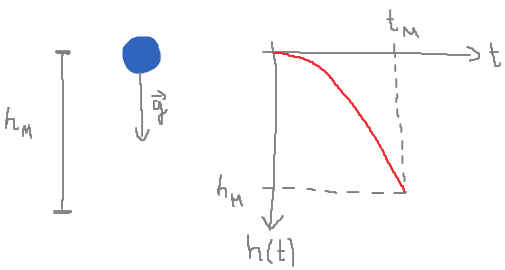
\includegraphics[width=0.6\textwidth]{freier-fall.png}
       \caption{Freier Fall mit zugehörigem h(t)-Diagramm} 
\end{figure} 
Beim freien Fall aus einer Höhe $h_M$ wirkt auf den Ball die Erdbeschleunigung $g=9.81 \frac{m}{s^2}$. Wir wählen unser Koordinatensystem so, dass der Ursprung im Ball liegt, und die positive Achse nach unten zeigt. In diesem System ist $s_0 = 0$, $g$ positiv und $h(t)$ wächst mit der Zeit. Wir betrachten jetzt nur Fälle, in denen $v_0 = 0 \frac{m}{s}$ gilt, als Übung bietet es sich jedoch an, die Formeln auch nochmal für gegebene $v_0 > 0$ aufzustellen und zu lösen. \\\\
Die charakteristischen Größen dieser Bewegung sind $a = g$, $v_0 = 0$, $h_M$ und $t_M$, wobei $t_M$ die Zeit ist, zu der der Ball landet. Aus $h_M$ können wir stets $t_M$ ermitteln, die Rückrichtung funktioniert ebenso: 
\begin{equation*}
    h(t_M) = h_M = \frac{g}{2}t_M^2 \Longleftrightarrow t_M = \sqrt{\frac{2h_M}{g}}
\end{equation*}
Bei bekannter Flugdauer $t_M$ (oder bekannter Fallhöhe $h_M$) finden wir auch direkt die Endgeschwindigkeit $v_M$: 
\begin{equation*}
    v(t_M) = v_M = gt_M = g\sqrt{\frac{2h_M}{g}} = \sqrt{\frac{2g^2h_M}{g}} = \sqrt{2gh_M}
\end{equation*}
In Aufgaben zum freien Fall können auch andere Kombinationen von Größen gegeben sein, z.B. könnte eine Aufgabe sein, aus gegebener Falldauer, Fallhöhe und Erdbeschleunigung eine Anfangsgeschwindigkeit $v_0 \neq 0$ zu ermitteln. Der Ansatz ist bei dieser Art von Kinematikaufgaben jedoch fast immer der gleiche - wir wählen ein Koordinatensystem, sodass möglichst viele Größen wegfallen oder entlang der Achsen zeigen (dann müssen wir sie nicht zerlegen), wir überlegen uns die wirkenden Beschleunigungen, die bestehenden Geschwindigkeiten und ihre Richtungen und zum Schluss stellen wir die Bewegungsgleichungen auf, die wir dann nach der gesuchten Größe auflösen. 

\section{Senkrechter Wurf}
Beim senkrechten Wurf werfen wir einen Ball mit einer Geschwindigkeit $v_0$ aufwärts, es wirkt die Erdbeschleunigung $g$. Der Ball steigt dann in der Zeit $t_M$ bis zu einer bestimmten Höhe $h_M$ auf, die Bewegung dreht sich dann um und der Ball fällt wieder nach unten. 
\begin{figure}[H] 
    \centering
       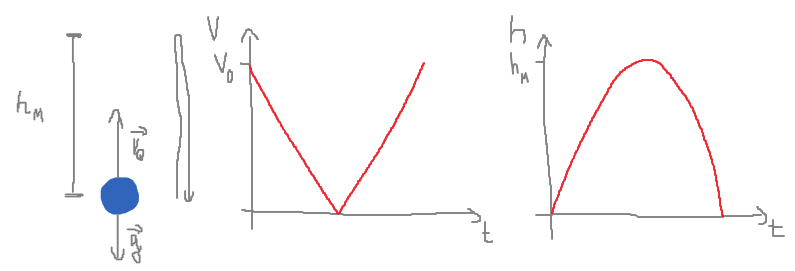
\includegraphics[width=\textwidth]{senkrechter-wurf.png}
       \caption{Senkrechter Wurf mit zugehörigem v(t)- und h(t)-Diagramm}
\end{figure} 
Hier müssen wir beachten, dass $v_0$ und $g$ in entgegengesetzte Richtungen zeigen, das passen wir durch die Vorzeichen in den Gleichungen an. Wir wählen unseren Koordinatenursprung wieder im Ball (also $s_0 = 0$), die positive Achse zeigt aber diesmal nach oben. \\\\
Bei Kinematikaufgaben kann man oftmals einen charakteristischen Punkt betrachten, hier bietet sich die Zeit $t_M$ an, da wir dort die Geschwindigkeit kennen. Sie ist 0. Damit können wir aus $v_0$ direkt $t_M$ ermitteln, und entsprechend auch aus $t_M$ $v_0$. 
\begin{equation*}
    v(t_M) = 0 = -gt_M + v_0 \Longleftrightarrow t_M = \frac{v_0}{g} \Longleftrightarrow v_0 = gt_M 
\end{equation*}
Zum Verständnis solltet ihr euch überlegen, was die physikalischen Aussagen dieser Gleichungen sind, und warum diese legitim erscheinen. Bei bekanntem $t_M$ können wir direkt die maximale Höhe $t_M$ finden.
\begin{equation*}
    h(t_M) = h_M = \frac{-g}{2}t_M^2 + v_0t_M = \frac{-g}{2}\frac{v_0^2}{g^2} + v_0\frac{v_0}{g} = \frac{-v_0^2}{2g}+\frac{v_0^2}{g} = \frac{v_0^2}{2g}
\end{equation*}
Damit können wir auch aus der Flughöhe auf die Anfangsgeschwindigkeit schließen.
\begin{equation*}
    h_M = \frac{v_0^2}{2g} \Longleftrightarrow v_0 = \sqrt{\frac{h_M}{2g}}
\end{equation*}
Wenn sich die Bewegung nun umdreht und der Ball wieder fällt ist der Fall komplett symmetrisch zum Aufstieg, wir landen genau nach der Zeit $t_M$ wieder auf dem Boden, damit ist die Gesamtflugdauer also $2t_M$. Die erreichte Endgeschwindigkeit ist gleich der Anfangsgeschwindigkeit. Als Übung könnt ihr das auch nochmal mit den Bewegungsgleichungen nachrechnen. 

\section{Schräger Wurf}
Beim schrägen Wurf werfen wir einen Ball mit der Geschwindigkeit $v_0$ im Winkel $\alpha$ zur Horizontalen ab, dabei durchläuft er zwei Teilbewegungen jeweils in x- und y-Richtung. Unter Vernachlässigung der Luftreibung bewegt er sich in x-Richtung mit der konstanten Geschwindigkeit $v_{x, 0}$ und in y-Richtung mit der konstanten Beschleunigung $-g$ und Anfangsgeschwindigkeit $v_{y, 0}$. 
\begin{figure}[H] 
    \centering
       \includegraphics[width=0.7\textwidth]{schräger-wurf.png}
       \caption{Schräger Wurf mit Zerlegung des Geschwindigkeitsvektors}
\end{figure} 
$v_{x, 0}$ und $v_{y, 0}$ finden wir mithilfe der trignometrischen Funktionen: 
$$v_{x, 0} = v_0\cos\alpha \quad\quad v_{y, 0} = v_0\sin\alpha$$
Hier ist es wichtig nachzuvollziehen, wieso dies der Fall ist - schaut euch wenn nötig nochmal das Trigonometrie-Skript an. Beachtet auch, dass das Zerlegungdreieck in Abb. 3 rechtwinklig ist, $v_{y, 0}$ ist senkrecht zur Horizontalen und $v_{x, 0}$ parallel dazu. 
\begin{figure}[H] 
    \centering
       \includegraphics[width=0.8\textwidth]{schräger-wurf-y.png}
       \caption{Diagramme zur y-Komponente des schrägen Wurfs}
\end{figure} 
Die Bewegung in y-Richtung entspricht genau einem senkrechten Wurf mit Anfangsgeschwindigkeit $v_0\sin\alpha$. Mit den in Abschnitt 2 hergeleiteten Formeln finden wir damit Maximalhöhe $\displaystyle h_M = \frac{v_0^2\sin^2\alpha}{2g}$, Dauer bis zum erreichen der Maximalhöhe $\displaystyle t_M = \frac{v_0\sin\alpha}{g}$ und Flugdauer $\displaystyle t_F = 2t_M = \frac{2v_0\sin\alpha}{g}$. Als Übung solltet ihr dies auch aus den Bewegungsgleichungen herleiten. 

\begin{figure}[H] 
    \centering
       \includegraphics[width=0.8\textwidth]{schräger-wurf-x.png}
       \caption{Diagramme zur x-Komponente des schrägen Wurfs}
\end{figure} 
Die Flugweite $w$ in x-Richtung berechnet sich zu 
\begin{equation*}
    s(t_F) = w = v_{x, 0}t_M = v_0\cos\alpha\frac{2v_0\sin\alpha}{g}
\end{equation*}
Es gilt 
$$\sin\alpha\cos\alpha = \frac{1}{2} \sin2\alpha$$
Als Übung zur Winkelsummenidentität solltet ihr das beweisen. Mit der trigonometrischen Identität gilt dann
$$w=\frac{v_0}{g}\sin2\alpha$$
$\sin\theta$ ist für $\theta = 90$° am größten (überlegt euch das am Einheitskreis), $w$ ist damit für $2\alpha=90$°, also $\alpha = 45$° maximal. \\\\
Stellen wir nun nochmal die Bewegungsgleichungen für beide Richtungen auf: 
\begin{gather}
    s_x(t) = v_0\cos\alpha t \Longleftrightarrow t = \frac{s_x(t)}{v_0\cos\alpha} \\
    h(t) = \frac{-g}{2}t^2 + v_0\sin\alpha t  
\end{gather}
Wir können (1) nun in (2) für die Zeit einsetzen: 
\begin{equation}
    h(s_x) = \frac{-g}{2}\frac{s_x^2(t)}{v_0^2\cos^2\alpha} + v_0\sin\alpha\frac{s_x(t)}{v_0\cos\alpha} = \frac{-g}{2v_0^2\cos^2\alpha}s_x^2(t) +\tan\alpha s_x(t)
\end{equation}
Dies ist eine quadratische Gleichung, die Höhe in Abhängigkeit von der Weite bildet damit eine umgedrehte Parabel (der Term vor $s_x^2(t)$ ist negativ). Das begründet auch die andere Bezeichnung des schrägen Wurfs - Parabelwurf. \\\\
Als allgemeine Anmerkung: obwohl das Einprägen einiger dieser Gleichungen womöglich bei einigen Aufgaben Zeit sparen könnte, ist es viel wichtiger, diese aus den Bewegungsgleichungen und Symmetrien herleiten zu können. 

\end{document}